\section{Introduction}
\label{sec:introduction}

In 1859, Michael Thonet patented chair No.\ 14: six steam-bent beechwood components, joined by ten screws and two nuts. The design was so efficient that 36 disassembled chairs fit in a single cubic meter for shipping. By 1930, over fifty million had been produced. The chair remains in continuous production today. Why this form?

The standard answer; ``form follows function'' \parencite{Sullivan1896}; fails on inspection. The function of a chair is to afford sitting to a human body. But this affordance is shared by every chair ever made: the Windsor, the Wassily, the Eames Lounge, the monobloc plastic garden chair. Sitting is constant across the class. It explains why chairs exist but carries zero information about why one chair takes one form rather than another \parencite{Michl1995}. If function determined form, all chairs would be identical. They are not.

This paper proposes a formal theory that answers the question. We call it \formlaere{} (Norwegian: \textit{theory of form}). The theory is structured as seven propositions that build from foundational definitions to an ethical conclusion:

\begin{enumerate}
\item The world of form is all that is the case.
\item Not all positions are equally probable.
\item The selection pressures produce a landscape.
\item The landscape is dynamic.
\item Agents exist.
\item Form arises between agents.
\item Form shows how far care reached.
\end{enumerate}

The theory synthesizes three formal traditions that have developed independently: George Stiny's shape algebra and form grammars \parencite{Stiny1972, Stiny2006}, which provide the \textit{syntax} of form; Armand Hatchuel and Benoit Weil's C-K theory \parencite{Hatchuel2003, Hatchuel2009}, which provides the \textit{epistemic logic} of the design process; and Michael Levin's multi-scale competence framework \parencite{Levin2022, Fields2022, Doctor2024}, which provides the \textit{dynamics} of agent-driven form production. The synthesis produces a single generative equation:

\begin{equation*}
\mathrm{Form} = SG\!\left(\nabla_{C(A)}\, L(c,\, t)\right)
\end{equation*}

\noindent Form is the grammar's response to the landscape gradient as perceived through the agent's cognitive cone. The theory introduces \textit{care}; the dimensionality of the agent's representational capacity; as the measure of design intelligence.

\subsection{The problem: ungrounded evaluation criteria}

Design theory currently evaluates theoretical proposals on criteria such as ``logic,'' ``correctness,'' ``clarity,'' and ``originality.'' These criteria, while reasonable in isolation, lack grounding in a shared formal framework. What counts as ``correct'' in design theory? Correct relative to what formal structure? What counts as ``original'' if there is no shared map of the theoretical landscape?

The consequence is that design theory operates without consensus on its own foundations. Shape grammars describe the syntax of form but do not explain why forms arise. C-K theory describes the logic of design reasoning but provides no morphological structure. Fitness landscape models from evolutionary biology explain pattern formation but have not been formalized for designed artifacts. And recent work on multi-scale agency and care \parencite{Doctor2024} provides a compelling account of intelligence as dimensional attention but has not been connected to design practice.

\subsection{Contribution}

This paper makes three contributions:

\begin{enumerate}
\item \textbf{Theoretical.} We present a formal design theory that unifies shape algebra, C-K theory, and multi-scale competence into a single framework. The theory is expressed as seven falsifiable propositions with a core generative equation.

\item \textbf{Empirical.} We test the theory against a corpus of 2,066 European chairs (1280--2024) drawn from two museum collections, with 2,204 supplementary three-dimensional mesh models. Twenty statistical analyses across 84 cross-validation tests confirm the theory's core predictions; no postulate is falsified.

\item \textbf{Practical.} We demonstrate the theory's explanatory reach through five worked examples spanning historical design (the cantilever chair race of 1925--1928), bio-fabrication (Neri Oxman's Silk Pavilion), AI-assisted design (Figma Weave), conversational agent design, and continental-scale ecological restoration (the Great Green Wall). Each example is described in concrete factual detail, not as a hypothetical illustration.
\end{enumerate}

\begin{figure*}[!t]
\centering
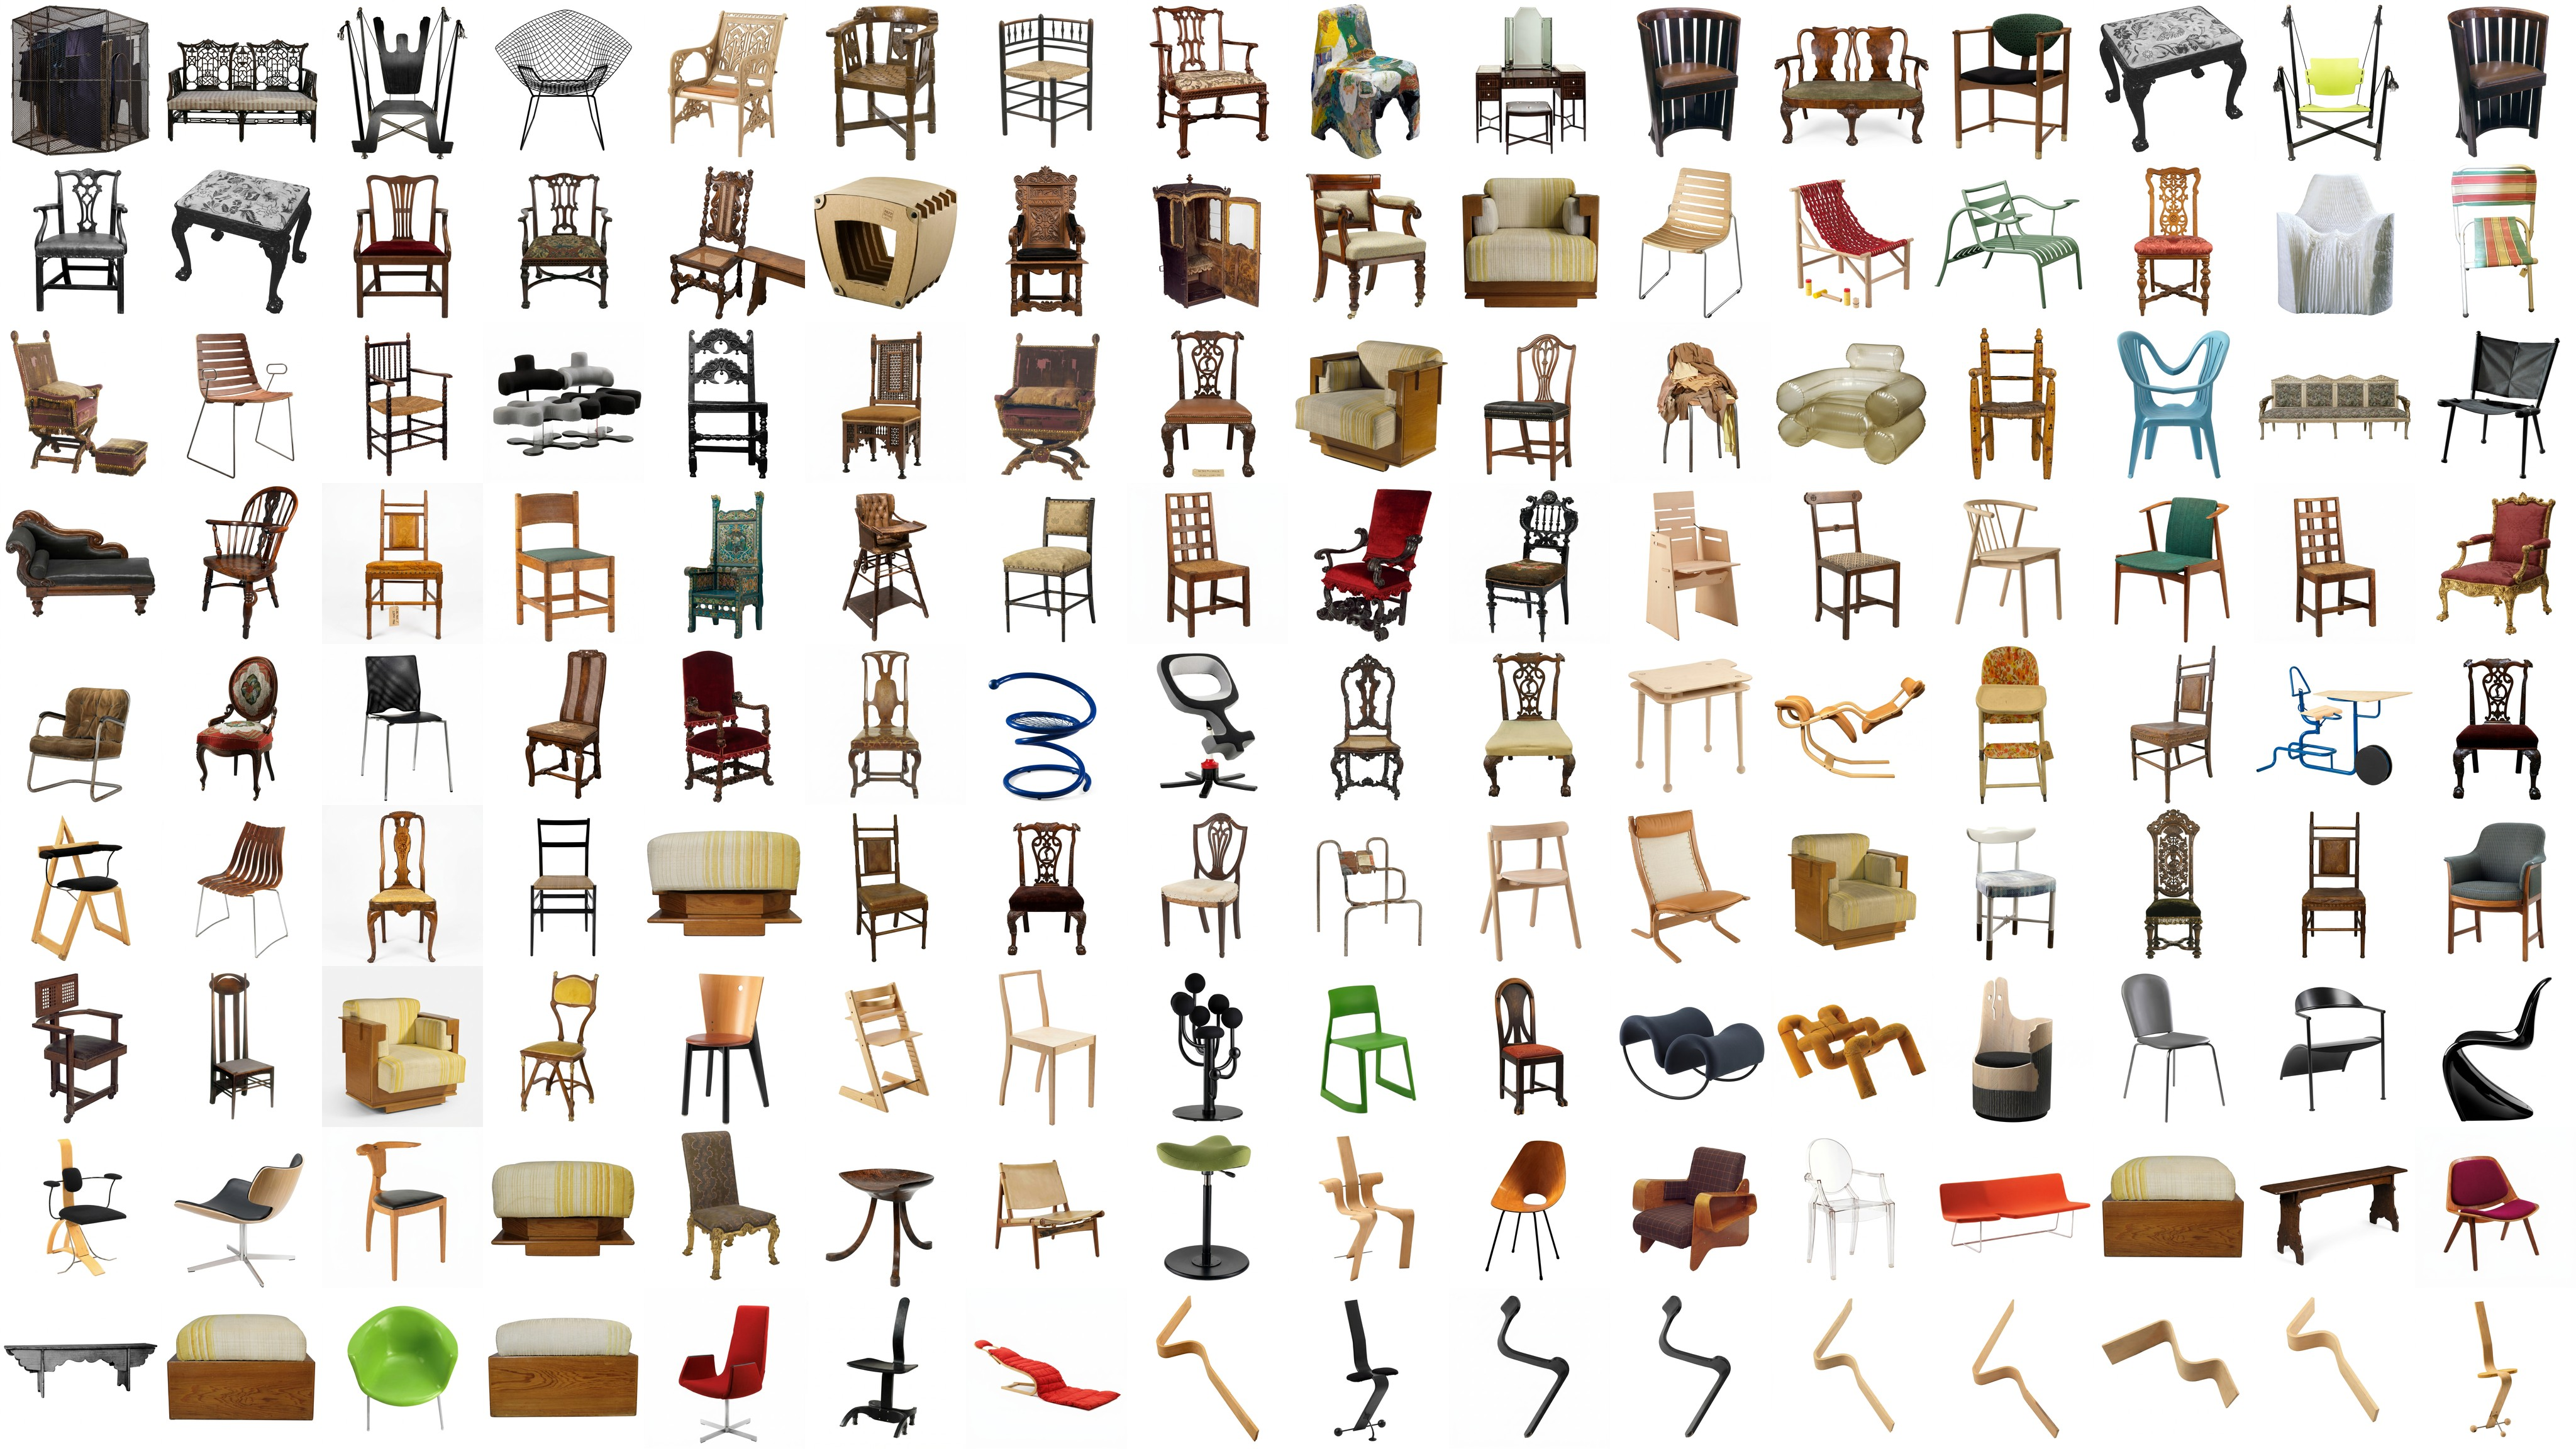
\includegraphics[width=\textwidth]{figures/chairs_top144_16x9.jpg}
\caption{A sample of 144 chairs from the corpus of 2,066 European chairs (1280--2024). The morphological diversity visible here; from medieval joined oak to postmodern plywood to contemporary injection-molded plastic; is the empirical phenomenon the theory seeks to explain.}
\label{fig:corpus}
\end{figure*}

The paper proceeds as follows. Section~\ref{sec:background} reviews the three source traditions and identifies the synthesis gap. Section~\ref{sec:theory} presents the seven propositions with formal definitions and the core equation. Section~\ref{sec:empirical} tests the theory empirically. Section~\ref{sec:examples} applies the theory to five worked examples. Section~\ref{sec:discussion} discusses explanatory power and limitations. Section~\ref{sec:agenda} proposes seven falsifiable research programs. Section~\ref{sec:conclusion} concludes.
